\usetikzlibrary{patterns}
\usetikzlibrary{arrows}

% Adapted from the 'patterns' library: enlarged the distance between the lines from 4pt to 10pt
\pgfdeclarepatternformonly{north east lines wide}{\pgfqpoint{-1pt}{-1pt}}{\pgfqpoint{10pt}{10pt}}{\pgfqpoint{9pt}{9pt}}%
{
  \pgfsetlinewidth{0.4pt}
  \pgfpathmoveto{\pgfqpoint{0pt}{0pt}}
  \pgfpathlineto{\pgfqpoint{9.1pt}{9.1pt}}
  \pgfusepath{stroke}
}


\tikzset{%
    body/.style={inner sep=0pt,outer sep=0pt,shape=rectangle,draw,thick,pattern=north east lines wide},
    dimen/.style={<->,>=latex,thin,every rectangle node/.style={fill=white,midway,font=\sffamily}},
    symmetry/.style={dashed,thin},
}

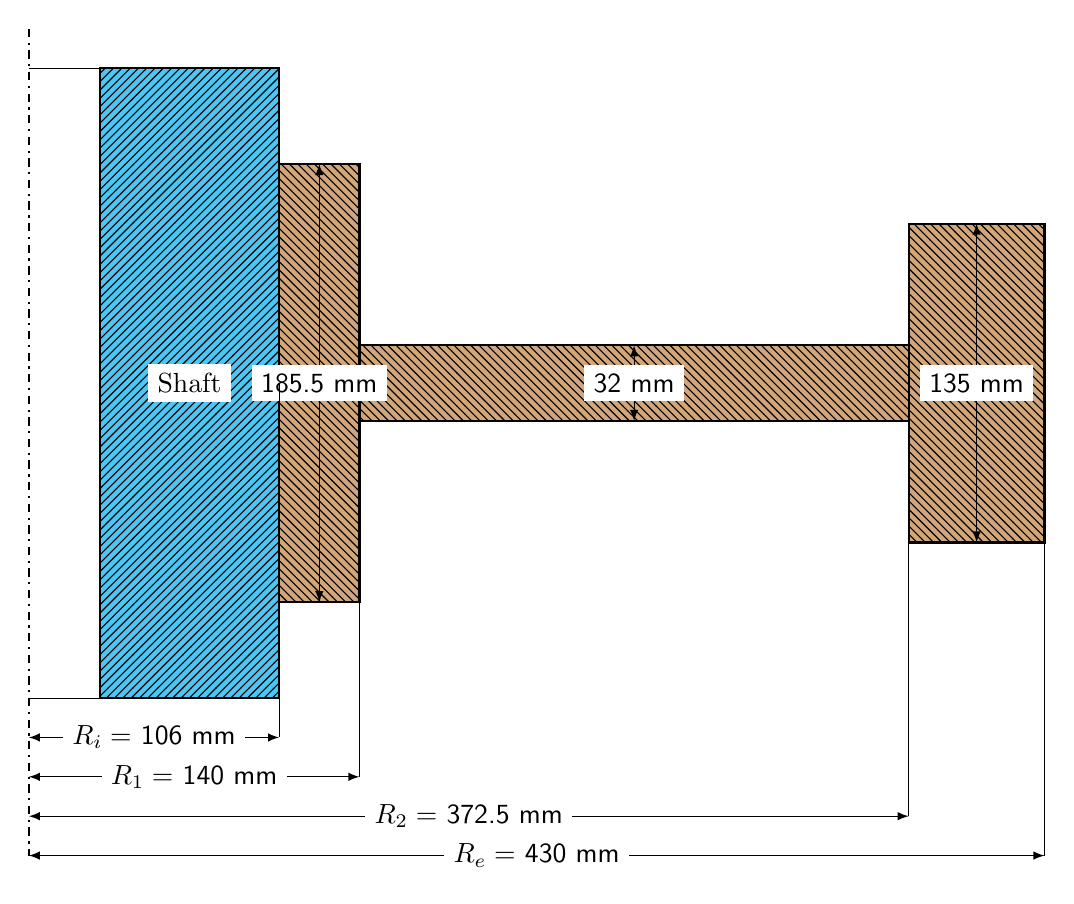
\begin{tikzpicture}
	
	\draw[thick,dashdotted] (0,4.5)--(0,-6);
	
	\def \k {3/100}
	
	%guide lines
	\draw[]  (0,4) -- (106*\k,4);
	\draw[]  (0,-4) -- (106*\k,-4);
	%%%%%%%%%%%%%%%%%%%
	
	\draw[thick,fill=cyan!70]  (30*\k,-4) rectangle (106*\k,4);
	\draw[thick,fill=brown!70]  (106*\k,-0.5*185.5*\k) rectangle (140*\k,0.5*185.5*\k);
	\draw[thick,fill=brown!70]  (140*\k,-0.5*32*\k) rectangle (372.5*\k,0.5*32*\k);
	\draw[thick,fill=brown!70]  (372.5*\k,-0.5*135*\k) rectangle (430*\k,0.5*135*\k);
	
	\draw[thick,pattern=north east lines]  (30*\k,-4) rectangle (106*\k,4) node[pos=.5,fill=white] {Shaft};
	\draw[thick,pattern=north west lines]  (106*\k,-0.5*185.5*\k) rectangle (140*\k,0.5*185.5*\k);
	\draw[thick,pattern=north west lines]  (140*\k,-0.5*32*\k) rectangle (372.5*\k,0.5*32*\k);
	\draw[thick,pattern=north west lines]  (372.5*\k,-0.5*135*\k) rectangle (430*\k,0.5*135*\k);
	
%	\draw[thick,pattern=north west lines]  (106*\k,-3) rectangle (140*\k,3);
%	\draw[thick,pattern=north west lines]  (140*\k,-3) rectangle (372.5*\k,3);
	
	\draw[dimen]  (0,-4.5) -- (106*\k,-4.5) node{$R_i=$ 106 mm};
	\draw[dimen]  (0,-5) -- (140*\k,-5) node {$R_1=$ 140 mm}; 
	\draw[dimen]  (0,-5.5) -- (372.5*\k,-5.5) node {$R_2=$ 372.5 mm}; 
	\draw[dimen]  (0,-6) -- (430*\k,-6) node {$R_e=$ 430 mm}; 
	
	
	\draw[dimen]  (246*0.5*\k,-0.5*185.5*\k) -- (246*0.5*\k,0.5*185.5*\k) node {185.5 mm}; 
	\draw[dimen]  (512.5*0.5*\k,-0.5*32*\k) -- (512.5*0.5*\k,0.5*32*\k) node {32 mm}; 
	\draw[dimen]  (802.5*0.5*\k,-0.5*135*\k) -- (802.5*0.5*\k,0.5*135*\k) node {135 mm}; 
	
	%guide lines
	\draw[] (106*\k,0) -- (106*\k,-4.5);
	\draw[] (140*\k,-1) -- (140*\k,-5);
	\draw[] (372.5*\k,0) -- (372.5*\k,-5.5);
	\draw[] (430*\k,0) -- (430*\k,-6);
	%%%%%%%%%%%%%%%%%%%%
	
\end{tikzpicture}